\documentclass[11pt]{article}
\usepackage[a4paper,margin=1in]{geometry}
\usepackage{microtype}
\usepackage{setspace}
\usepackage{booktabs,tabularx,array,multirow}
\usepackage{amsmath,amssymb,amsthm,mathtools}
\usepackage{graphicx}
\usepackage{tikz}
\usetikzlibrary{arrows.meta,positioning,shapes.geometric,fit}
\usepackage{pgfplots}
\pgfplotsset{compat=1.18}
\usepackage{algorithm}
\usepackage{algpseudocode}
\usepackage{hyperref}
\usepackage[nameinlink,noabbrev]{cleveref}
\usepackage[backend=biber,style=apa,sorting=nyt,maxbibnames=99]{biblatex}
\DeclareLanguageMapping{english}{english-apa}
\addbibresource{references.bib}
\usepackage{xcolor}
\usepackage{enumitem}
\usepackage{caption}
\usepackage{csquotes}

\hypersetup{colorlinks=true,linkcolor=black,citecolor=blue,urlcolor=blue}
\setstretch{1.08}
\newtheorem{theorem}{Theorem}
\newtheorem{definition}{Definition}
\newtheorem{proposition}{Proposition}
\newcommand{\cA}{\mathcal{A}}
\newcommand{\cW}{\mathcal{W}}
\newcommand{\cE}{\mathcal{E}}
\newcommand{\RBE}{\textsc{RBE}}

\title{\textbf{Beyond Outcome Attainment: Resolution-Based Education and the Certification--Assessment Resolution Gap in the Generative-AI Era}}
\author{Mohammad Amir Khusru Akhtar\\Usha Martin University, Ranchi, India}
\date{}

\begin{document}
\maketitle

\begin{abstract}
Generative artificial intelligence can produce polished academic artifacts while leaving uncertain which capabilities belong to the learner. This creates a certification problem deeper than plagiarism detection: two learners can generate observationally similar work while requiring different certification decisions. We formalize this problem as the \emph{Certification--Assessment Resolution Gap} (CARG). An assessment protocol induces equivalence classes over learner worlds; valid certification requires that every equivalence class be homogeneous with respect to the intended certification decision. We prove a necessity result: if two assessment-indistinguishable worlds require different certification decisions, no rule based only on that protocol can be universally correct. We then introduce Resolution-Based Education (RBE), which augments outcome-based assessment with adaptive, low-burden perturbations designed to restore decision-relevant resolution. The operational objective is not maximal questioning, but the cheapest experiment that separates still-compatible, certification-incompatible worlds. Reproducible software tests include deterministic and probabilistic benchmarks, 20,000 Monte Carlo episodes, and retrospective evaluation on 32,593 Open University student-module records. Falsification controls reject a broad claim of predictive superiority: adaptive acquisition does not consistently beat strong confidence-based fixed evidence on selective risk. What survives is a sharper contribution---a formal certification-resolution criterion and evidence-efficient selective assessment that demonstrably reduces evidence burden while preserving risk thresholds.
\end{abstract}

\noindent\textbf{Keywords:} generative artificial intelligence; higher education assessment; certification validity; adaptive assessment; epistemic agency; evidence efficiency

\section{Introduction}
Universities do more than mark performances. They make consequential claims about what learners can understand, judge, verify, transfer, and responsibly do. Classical validity theory therefore treats assessment not as a property of a test form but as an evidentiary argument connecting observations to interpretations and decisions \parencite{messick1995validity}. Evidence-centered design similarly begins with the claim to be made, the evidence needed to support it, and the tasks capable of producing that evidence \parencite{mislevy2003ecd}. These foundations become unusually visible in the generative-AI era because the mapping from learner capability to observed work is no longer close to one-to-one.

The current literature has documented substantial pressures on higher-education assessment. Generative systems can produce fluent essays, code, explanations, solutions, and plausible feedback; policy responses have ranged from prohibition to redesign, while emerging research emphasizes authentic assessment, AI literacy, evaluative judgement, verification, and responsible tool use \parencite{unesco2023guidance,luo2024policies,xia2024scoping,yusuf2024future,kofinas2025authentic,khlaif2025redesign}. Yet the core inferential problem is more precise than ``AI makes cheating easier.'' A learner with deep understanding, a learner who can verify but not independently generate, and a learner who follows a plausible AI answer without understanding can sometimes produce essentially the same assessed artifact. If the credential intends to distinguish among those capability states, artifact quality alone may be insufficient.

This paper addresses a narrower question: \emph{when does an assessment protocol lack the resolution required by its own certification rule?} We call the resulting structural mismatch the \emph{Certification--Assessment Resolution Gap} (CARG). The idea is deliberately decision-relative. Assessment need not recover a learner's complete latent state; it only needs to distinguish still-compatible learner worlds when those worlds require different certification decisions. The central formal result is elementary but consequential: if a protocol makes two worlds observationally indistinguishable while the credential requires different decisions for them, no decision rule using only that protocol can always be correct.

From this condition we develop \emph{Resolution-Based Education} (RBE), an extension of outcome-based assessment rather than a rejection of it. Outcome specification remains essential. RBE adds a second question: \emph{does the available evidence resolve whether the claimed capability is actually certifiable?} If not, the response is not automatically a longer exam. The assessment should seek the minimum admissible perturbation---for example, a changed constraint, misleading recommendation, contradictory evidence, or transfer task---that separates certification-incompatible learner worlds still consistent with the evidence.

The paper makes five contributions. First, it formalizes CARG as a mismatch between the observational partition induced by assessment and the decision partition required by certification. Second, it proves a Certification Resolution Necessity result. Third, it defines a Minimum Resolution-Restoring Perturbation (MRRP) objective with burden and assessment leakage. Fourth, it develops a probabilistic, risk-constrained Resolution Engine and an educational architecture integrating curriculum, learning, assessment, and certification. Fifth, it subjects the framework to reproducible falsification: deterministic and probabilistic constructions, 20,000 noisy Monte Carlo episodes, and a retrospective OULAD analysis with matched-coverage confidence controls, random acquisition-order controls, and bootstrap uncertainty. The negative findings are retained. Adaptive RBE does not consistently dominate strong fixed evidence on selective prediction risk. The real-data contribution that survives is narrower: selective adaptive acquisition can reduce evidence burden substantially under the declared risk criterion.

\section{From Outcome Evidence to Certification Resolution}
\subsection{The inferential problem}
Let $W$ denote a set of possible learner worlds. A world is not a claim about an inaccessible mental essence; it is a modeling device representing educationally relevant capability configurations that can generate observable behavior. Let $g:W\to D$ be the required certification rule, where $D$ may be binary (certify/do not certify) or multicategorical.

An assessment protocol $\cA$ specifies the observations and interventions the institution permits: artifact inspection, oral defense, constraint shifts, tool restrictions, misleading AI suggestions, transfer tasks, evidence requests, and so forth. Two worlds are assessment-equivalent when the protocol cannot distinguish them.

\begin{definition}[Assessment equivalence]
For learner worlds $w_i,w_j\in W$, define
\[
 w_i\sim_{\cA}w_j
 \quad\Longleftrightarrow\quad
 \text{all evidence obtainable under }\cA\text{ is observationally indistinguishable between }w_i\text{ and }w_j.
\]
The relation $\sim_{\cA}$ induces an assessment partition $\Pi_{\cA}=W/\!\sim_{\cA}$.
\end{definition}

The certification rule $g$ induces a second partition $\Pi_g$, where worlds belong to the same cell when they receive the same certification decision. Certification is resolvable only when the assessment partition is at least as fine as the decision partition.

\begin{definition}[Certification--Assessment Resolution Gap]
A CARG exists under $(g,\cA)$ if there are worlds $w_i,w_j\in W$ such that
\[
 w_i\sim_{\cA}w_j
 \qquad\text{and}\qquad
 g(w_i)\neq g(w_j).
\]
Equivalently, $\Pi_{\cA}$ fails to refine $\Pi_g$.
\end{definition}

\Cref{fig:carg} makes the idea concrete. Four latent learner worlds can collapse to the same observed artifact even though the certification rule separates them.

\begin{figure}[t]
\centering
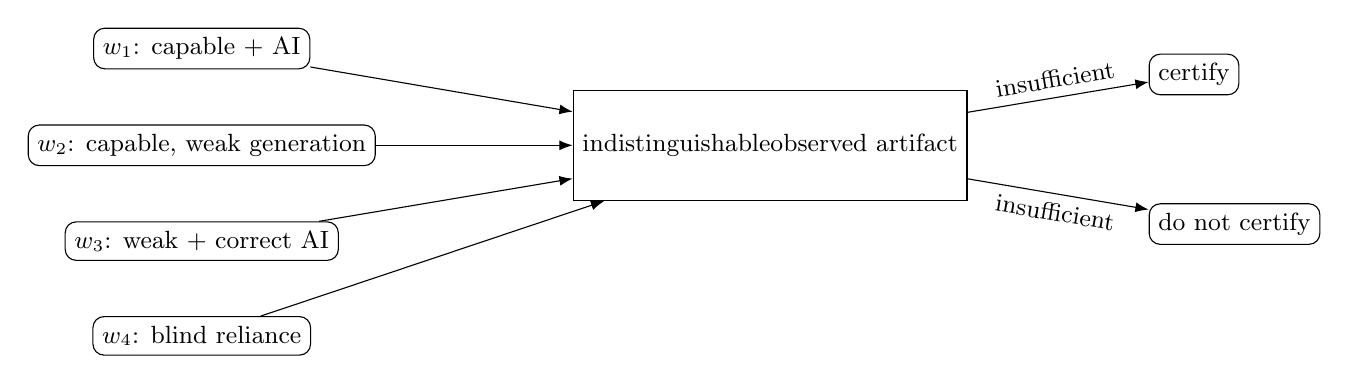
\begin{tikzpicture}[node distance=7mm and 15mm,>=Latex, every node/.style={font=\small}]
\node[draw,rounded corners] (w1) {$w_1$: capable + AI};
\node[draw,rounded corners,below=of w1] (w2) {$w_2$: capable, weak generation};
\node[draw,rounded corners,below=of w2] (w3) {$w_3$: weak + correct AI};
\node[draw,rounded corners,below=of w3] (w4) {$w_4$: blind reliance};
\node[draw,minimum width=34mm,minimum height=14mm,right=25mm of w2] (obs) {indistinguishable\\observed artifact};
\node[draw,rounded corners,right=23mm of obs,yshift=9mm] (c1) {certify};
\node[draw,rounded corners,right=23mm of obs,yshift=-10mm] (c0) {do not certify};
\foreach \x in {w1,w2,w3,w4}{\draw[->] (\x) -- (obs);}
\draw[->] (obs) -- node[above,sloped]{insufficient} (c1);
\draw[->] (obs) -- node[below,sloped]{insufficient} (c0);
\end{tikzpicture}
\caption{CARG in an artifact-only assessment. Different learner worlds can collapse to the same observed artifact even though the certification rule requires different decisions. Source: authors' formal construction.}
\label{fig:carg}
\end{figure}

\subsection{Certification Resolution Necessity}
\begin{theorem}[Certification Resolution Necessity]
Let $\cA$ be an assessment protocol and $g:W\to D$ the intended certification rule. If there exist $w_i,w_j\in W$ such that $w_i\sim_{\cA}w_j$ and $g(w_i)\neq g(w_j)$, then no decision function based exclusively on evidence obtainable under $\cA$ can be universally correct with respect to $g$.
\end{theorem}

\begin{proof}
Because $w_i\sim_{\cA}w_j$, the complete $\cA$-observable evidence is identical (or, in the stochastic extension, identically distributed) in the two worlds. Any decision function receiving only that evidence must therefore return the same decision for both. But $g(w_i)\neq g(w_j)$, so at least one returned decision must disagree with $g$. Hence universal correctness is impossible.
\end{proof}

The deterministic theorem is deliberately a necessity result, not a novelty claim about equivalence relations. The contribution is its explicit role as a certification-validity condition. In deterministic settings it also yields a simple sufficiency statement: if $g$ is constant on every assessment-equivalence class, a decision rule can be defined on each class by its common $g$ value.

\section{Minimum Resolution-Restoring Perturbations}
Exact identification of a learner world is often unnecessary. If several remaining worlds all imply the same certification decision, further testing may add burden without decision value. RBE therefore seeks perturbations that distinguish \emph{cross-decision} worlds.

Let $K_t$ denote current knowledge after $t$ observations and $W(K_t)\subseteq W$ the compatible worlds. Let an admissible perturbation $e\in\cE$ have direct burden $c(e)$ and assessment leakage $L(e)$, where leakage represents capability-relevant information supplied by the assessment itself. A simple burden model is
\[
 B_\lambda(e)=c(e)+\lambda L(e),\qquad \lambda\ge 0.
\]
For deterministic separation, define $e$ to be resolving for a set of cross-decision pairs if their predicted observations under $e$ are disjoint.

\begin{definition}[Minimum Resolution-Restoring Perturbation]
Given current knowledge $K_t$, an MRRP is
\[
 e_t^*\in\arg\min_{e\in\cE} B_\lambda(e)
\]
subject to a declared resolution condition over the certification-incompatible worlds remaining in $W(K_t)$.
\end{definition}

The phrase ``cheapest experiment'' therefore never means merely ``the lowest-cost question.'' A very cheap probe can be useless if it leaves decision-incompatible worlds observationally merged. \Cref{alg:det} gives the deterministic mechanism.

\begin{algorithm}[t]
\caption{Minimum Resolution-Restoring Perturbation (deterministic form). Source: authors' RBE implementation.}
\label{alg:det}
\begin{algorithmic}[1]
\Require Compatible worlds $W$, certification rule $g$, probes $\cE$, leakage weight $\lambda$
\State Construct unresolved pairs $P=\{(w_i,w_j):g(w_i)\neq g(w_j)\}$
\For{each $e\in\cE$}
  \State Compute burden $B_\lambda(e)=c(e)+\lambda L(e)$
  \State Test whether $e$ separates every pair in $P$
\EndFor
\State Discard non-resolving probes
\State \Return resolving probe with minimum $B_\lambda(e)$
\end{algorithmic}
\end{algorithm}

\subsection{Probabilistic resolution and selective decisions}
Real assessment responses are noisy. Let $D=g(W)$ be the certification decision and $Y_e$ the response to perturbation $e$. One useful decision-relative quantity is the expected reduction in certification entropy,
\[
 IG_D(e)=H(D)-\mathbb{E}_{Y_e}[H(D\mid Y_e)],
\]
with entropy $H$ in the Shannon sense \parencite{shannon1948}. The cheapest informative perturbation at threshold $\tau$ is
\[
 e^*\in\arg\min_e B_\lambda(e)
 \quad\text{s.t.}\quad
 IG_D(e)\ge \tau.
\]
This is an application of established information and experiment-design ideas rather than a claim of new generic mathematics \parencite{lindley1956,blackwell1953,settles2009}.

For certification, posterior decision risk is often more directly interpretable. For binary $D$ and posterior $p_t=P(D=1\mid K_t)$, define
\[
 r_t=\min(p_t,1-p_t).
\]
An adaptive policy can stop and certify or reject when $r_t\le\epsilon$, while abstaining or acquiring another perturbation otherwise. Selective prediction and reject-option classification provide established statistical ancestors for such risk--coverage trade-offs \parencite{chow1970,elyaniv2010,gangrade2021}. RBE supplies the educational object being resolved: certification-relevant learner-world distinctions.

\section{Resolution-Based Education}
RBE extends rather than replaces outcome-oriented and evidence-centered assessment. Outcome specifications remain necessary, but an outcome statement alone does not establish that a particular assessment can resolve the capability distinction implied by the credential. The proposed architecture adds a certification-resolution layer to constructive alignment, evidence-centered design, authentic assessment, adaptive expertise, and dynamic assessment \parencite{biggs1996alignment,mislevy2003ecd,gulikers2004authentic,hatano1986adaptive,allal2000zpd}.

At curriculum level, a \emph{Resolvable Capability Outcome} specifies (i) the capability claim, (ii) the environments in which it must hold, including legitimate tool use, (iii) admissible perturbations, and (iv) the certification distinction that matters. At learning level, AI, search, software, calculators, peers, and feedback can remain legitimate developmental resources. At certification level, the question is whether the evidence supports the required inference.

A short \emph{Resolution Episode} follows the sequence
\[
 \text{Produce}\rightarrow\text{Perturb}\rightarrow\text{Explain}\rightarrow\text{Verify}\rightarrow\text{Adapt}.
\]
A perturbation need not remove AI. It may instead make the AI wrong, incomplete, overconfident, or inconsistent with new evidence, thereby testing whether the learner can appropriately trust, challenge, verify, or revise external support. This focus is compatible with work on evaluative judgement, AI literacy, verification, and appropriate reliance \parencite{bearman2024evaluative,tzirides2024ailiteracy,fok2024verifiability,passi2024reliance}.

\begin{figure}[t]
\centering
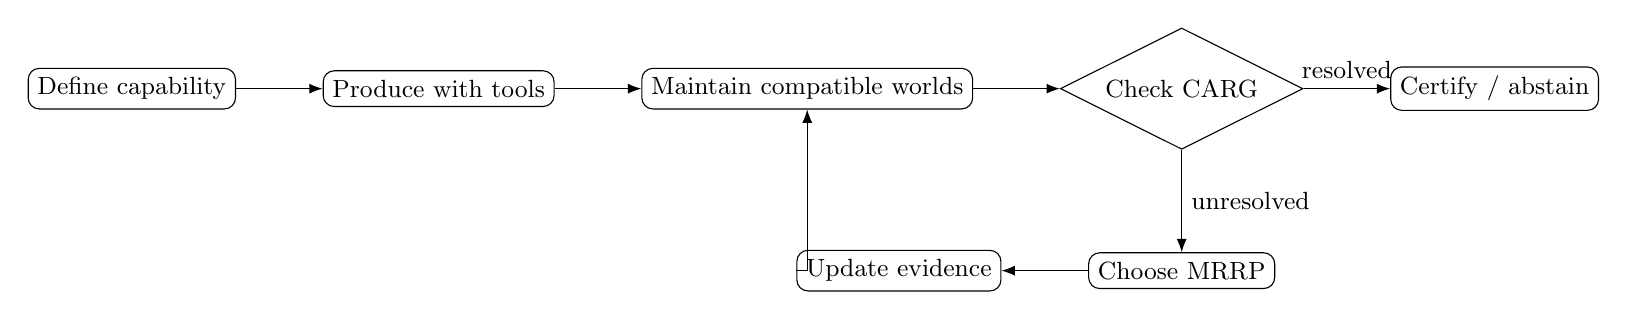
\begin{tikzpicture}[node distance=10mm and 11mm,>=Latex,every node/.style={font=\small}]
\node[draw,rounded corners] (claim) {Define capability};
\node[draw,rounded corners,right=of claim] (prod) {Produce with tools};
\node[draw,rounded corners,right=of prod] (worlds) {Maintain compatible worlds};
\node[draw,diamond,aspect=2,right=of worlds] (gap) {Check CARG};
\node[draw,rounded corners,below=13mm of gap] (probe) {Choose MRRP};
\node[draw,rounded corners,left=of probe] (update) {Update evidence};
\node[draw,rounded corners,right=of gap] (cert) {Certify / abstain};
\draw[->] (claim)--(prod); \draw[->](prod)--(worlds); \draw[->](worlds)--(gap);
\draw[->] (gap)-- node[above]{resolved}(cert);
\draw[->] (gap)-- node[right]{unresolved}(probe);
\draw[->](probe)--(update); \draw[->](update)-|(worlds);
\end{tikzpicture}
\caption{RBE resolution engine. Assessment continues only while certification-incompatible worlds remain observationally compatible. Source: authors' systems design implemented in the RBE repository.}
\label{fig:engine}
\end{figure}

\Cref{fig:engine} operationalizes the framework. A production task yields evidence, the Resolution Engine maintains compatible worlds, checks whether the current observational classes are decision-homogeneous, and acquires additional evidence only when necessary.

\begin{algorithm}[t]
\caption{Adaptive Resolution Engine (risk-constrained form). Source: authors' RBE implementation and experiments.}
\label{alg:adaptive}
\begin{algorithmic}[1]
\Require Initial evidence $K_0$, worlds $W$, decision rule $g$, probes $\cE$, risk threshold $\epsilon$
\State $t\gets0$
\Loop
  \State Update compatible/posterior learner worlds from $K_t$
  \State Compute certification posterior and decision risk $r_t$
  \If{$r_t\le\epsilon$}
    \State \Return certification decision and resolved evidence trail
  \EndIf
  \If{no admissible probe can improve resolution}
    \State \Return abstain / unresolved
  \EndIf
  \State Choose minimum-burden admissible probe satisfying the desired resolution criterion
  \State Observe response and update $K_{t+1}$
  \State $t\gets t+1$
\EndLoop
\end{algorithmic}
\end{algorithm}

\section{Novelty Boundary and Relation to Prior Work}
The contribution is easiest to understand by stating what it does \emph{not} claim. Optimal experimental design, sequential testing, teaching dimension, query complexity, active learning, adaptive testing, and selective classification already provide methods for obtaining information efficiently \parencite{wald1947,settles2009,vanderlinden2010,gangrade2021}. Dynamic assessment has long treated interaction and graduated support as informative about developing capability \parencite{allal2000zpd,poehner2011validity}. Evidence-centered design and validity theory already insist that tasks and evidence be aligned to intended claims \parencite{mislevy2003ecd,messick1995validity}. Authentic assessment and evaluative judgement similarly emphasize realistic performance and learners' capacity to judge quality \parencite{gulikers2004authentic,bearman2024evaluative}.

RBE's proposed object is the pair consisting of a \emph{certification rule} and an \emph{assessment protocol}. CARG asks whether the protocol's observational partition is fine enough for the decision partition demanded by the credential. MRRP then instantiates established experiment-design principles against that specifically educational failure. \Cref{tab:boundary} summarizes the boundary.

\begin{table}[t]
\centering
\caption{Relations between RBE and established assessment/decision traditions. Source: authors' synthesis of cited literature.}
\label{tab:boundary}
\small
\begin{tabularx}{\textwidth}{p{.23\textwidth}p{.32\textwidth}X}
\toprule
Tradition & Established contribution & RBE-specific role / boundary \\
\midrule
Validity and ECD & Evidence supports interpretations and decisions; assessment as an evidentiary argument & Makes certification partitions explicit and asks whether observable classes refine them \\
Dynamic assessment & Learning/development revealed through supported interaction & Uses controlled perturbations for decision-relevant discrimination, not necessarily developmental diagnosis \\
Authentic assessment & Realistic tasks, multiple judgements, contextualized performance & Does not assume authenticity alone resolves attribution in AI-mediated work \\
Sequential/selective testing & Efficient information acquisition, stopping, abstention & Applies cost/risk logic to certification-incompatible learner worlds \\
Selective classification & Risk--coverage trade-offs & Supplies statistical machinery; RBE supplies the educational decision target \\
\bottomrule
\end{tabularx}
\end{table}

\section{Reproducible Computational Validation}
All experiments are implemented in the public repository listed in the Data and Code Availability section. Tests are designed to separate mechanism validation from human educational evidence. Synthetic results are never interpreted as real-student effects.

\subsection{Deterministic cheapest resolving experiment}
The first benchmark uses four constructed worlds. All produce the same artifact-level observation, so artifact-only assessment leaves four cross-decision pairs unresolved. Four perturbations are assigned declared burdens $B_\lambda(e)$ at $\lambda=1$.

A deliberately cheap wrong-AI check has burden 0.55 but does not separate every certification-incompatible pair. A constraint-shift perturbation has burden 1.10 and is a full separator; transfer has burden 1.25 and generic viva has burden 6.00. Thus the cheapest raw probe is not the cheapest \emph{feasible resolving} probe. \Cref{tab:deterministic,fig:detburden} show the result.

\begin{table}[t]
\centering
\caption{Deterministic resolving benchmark. ``Full separator'' means every currently unresolved cross-decision pair is separated. Source: RBE software benchmark and test registry.}
\label{tab:deterministic}
\begin{tabular}{lrrl}
\toprule
Probe & Burden & Full separator? & Role \\
\midrule
Wrong-AI check & 0.55 & No & Cheapest raw probe \\
Constraint shift & 1.10 & Yes & Cheapest feasible resolver \\
Transfer task & 1.25 & Yes & Feasible resolver \\
Generic viva & 6.00 & Yes & High-burden resolver \\
\bottomrule
\end{tabular}
\end{table}

\begin{figure}[t]
\centering
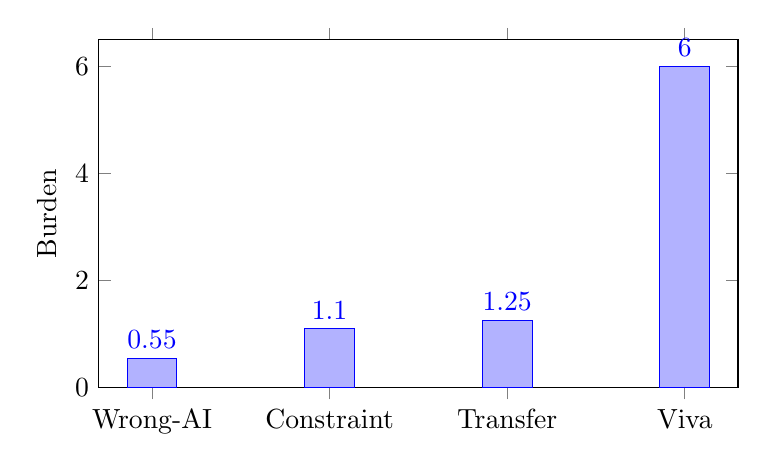
\begin{tikzpicture}
\begin{axis}[width=.8\textwidth,height=6cm,ybar,bar width=18pt,ylabel={Burden},symbolic x coords={Wrong-AI,Constraint,Transfer,Viva},xtick=data,ymin=0,ymax=6.5,nodes near coords]
\addplot coordinates {(Wrong-AI,0.55) (Constraint,1.10) (Transfer,1.25) (Viva,6.00)};
\end{axis}
\end{tikzpicture}
\caption{Declared burden of candidate probes in the deterministic benchmark. The cheapest raw probe is not a full separator; the constraint shift is the cheapest feasible resolver. Source: RBE deterministic benchmark.}
\label{fig:detburden}
\end{figure}

\subsection{Probabilistic benchmark}
The probabilistic version assigns each world a response probability for each probe. With equal prior mass on two certify and two non-certify worlds, initial decision entropy is one bit. Artifact-only evidence has zero decision information. A weak, low-burden probe can qualify at a modest threshold but fail a stronger decision-information requirement. The software therefore verifies the constrained form of ``cheapest experiment'': cost is minimized only among probes meeting a declared resolution standard.

\subsection{Monte Carlo falsification}
We next simulate 20,000 noisy learner episodes with seed 20260916. The adaptive sequence uses constraint shift, wrong-AI check, transfer, then generic viva, stopping when the posterior certification probability crosses 0.90 in either direction. A fixed targeted sequence and one generic viva provide controls. \Cref{tab:mc,fig:mc} report the saved result.

\begin{table}[t]
\centering
\caption{Monte Carlo mechanism test over 20,000 seeded synthetic episodes. Source: RBE workflow report \texttt{ADAPTIVE\_MONTE\_CARLO.md}.}
\label{tab:mc}
\begin{tabular}{lrrrr}
\toprule
Protocol & Resolved & Error/resolved & Mean burden & Mean probes \\
\midrule
Adaptive RBE & 0.9645 & 0.0861 & 2.4455 & 1.8261 \\
Fixed targeted & 0.7736 & 0.0645 & 2.0769 & 2.3415 \\
Generic viva & 0.4686 & 0.0768 & 6.0000 & 1.0000 \\
\bottomrule
\end{tabular}
\end{table}

\begin{figure}[t]
\centering
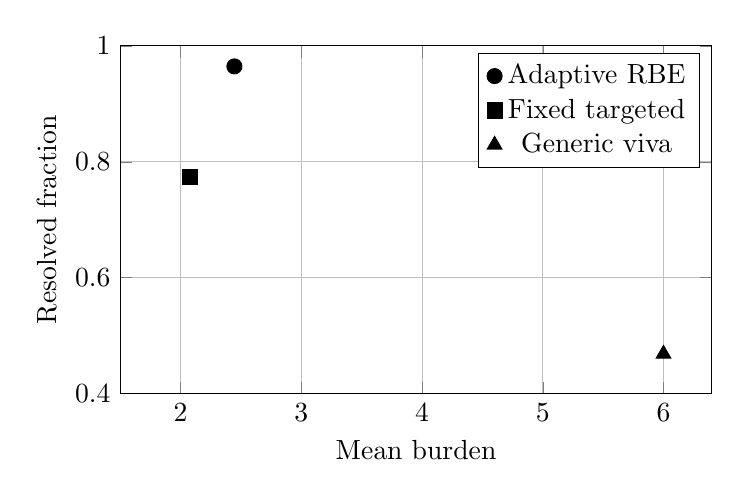
\begin{tikzpicture}
\begin{axis}[width=.75\textwidth,height=6cm,xlabel={Mean burden},ylabel={Resolved fraction},xmin=1.5,xmax=6.4,ymin=.4,ymax=1.0,grid=major]
\addplot[only marks,mark=*,mark size=2.7pt] coordinates {(2.4455,.9645)};
\addlegendentry{Adaptive RBE}
\addplot[only marks,mark=square*,mark size=2.7pt] coordinates {(2.0769,.7736)};
\addlegendentry{Fixed targeted}
\addplot[only marks,mark=triangle*,mark size=3pt] coordinates {(6,.4686)};
\addlegendentry{Generic viva}
\end{axis}
\end{tikzpicture}
\caption{Resolution--burden trade-off in the 20,000-episode Monte Carlo study. Source: RBE reproducible simulation.}
\label{fig:mc}
\end{figure}

The adaptive protocol resolves substantially more episodes and costs far less than a generic viva, but it does not dominate error. Error among resolved cases is 8.61\% for adaptive RBE versus 6.45\% for the fixed targeted sequence. This is a useful failure: maximizing resolution alone can over-resolve uncertain cases. The result motivates the risk-constrained form in \Cref{alg:adaptive} rather than a resolution-only objective.

\section{Retrospective Real-Data Study on OULAD}
\subsection{Dataset and design}
The Open University Learning Analytics Dataset (OULAD) contains 32,593 student-module records together with assessment data and 10,655,280 daily virtual learning environment interaction summaries \parencite{kuzilek2017oulad}. OULAD predates GenAI and was not collected under RBE. It is therefore used only as a retrospective proxy for adaptive evidence acquisition, not as causal evidence that RBE improves education or AI-era assessment.

We construct pre-cutoff evidence at days 60, 90, and 120: mean assessment score, assessment count, VLE clicks, active days, VLE record count, and submission lateness. Students are group-disjoint across train, validation, and test splits. Logistic models use median imputation with missingness indicators and standardized numerical features. The acquisition order is learned on validation data and then frozen. The target is eventual course outcome (Pass/Distinction versus other final outcomes). This target is an operational proxy, not a direct measure of capability.

\subsection{Fixed versus adaptive evidence}
At cutoff 120, the held-out all-outcomes test set contains $n=6{,}505$ student-module records. \Cref{tab:ouladmain} summarizes the principal comparison at $\epsilon=.20$.

\begin{table}[t]
\centering
\caption{OULAD held-out comparison at cutoff 120. Risk is classification error; adaptive-resolved risk is conditional on the resolved subset. Source: RBE workflow artifact \texttt{oulad-final-comparison-results}.}
\label{tab:ouladmain}
\small
\begin{tabular}{lrrrrr}
\toprule
Protocol & Coverage & Risk & Accuracy & AUC & Burden \\
\midrule
Score-only baseline & 1.000 & 0.2397 & 0.7603 & 0.8347 & 1.000 \\
Enhanced fixed all evidence & 1.000 & 0.2143 & 0.7857 & 0.8802 & 6.000 \\
RBE adaptive, resolved only & 0.5273 & 0.0880 & 0.9120 & --- & 3.633 \\
Fixed matched-budget prefix & 1.000 & 0.2161 & 0.7839 & 0.8792 & 4.000 \\
\bottomrule
\end{tabular}
\end{table}

The initial result in \Cref{tab:ouladmain} is intentionally not interpreted as ``8.8\% versus 21.4\%'' superiority, because the coverage differs. The adaptive protocol selectively resolves easier cases; direct comparison to a 100\%-coverage baseline would confound acquisition with abstention. Indeed, when RBE is forced to decide all cases, its classification risk equals the enhanced fixed-evidence risk (0.214297). This negative finding blocks a broad predictive-superiority claim.

\subsection{Matched-coverage and random-order falsification}
A stronger falsification compares RBE against fixed-all-evidence confidence selection at exactly the same coverage and against 100 random acquisition orders. \Cref{tab:falsification} reports the key cutoff-120 results.

\begin{table}[t]
\centering
\caption{Matched-coverage falsification at cutoff 120. Source: RBE workflow run 35071457218 and saved artifact \texttt{oulad\_selective\_falsification\_results.csv}.}
\label{tab:falsification}
\small
\begin{tabular}{llrrr}
\toprule
Population & Method & Risk & Coverage & Burden \\
\midrule
All, $\epsilon=.10$ & RBE adaptive & 0.02276 & 0.31068 & 4.582 \\
All, $\epsilon=.10$ & Fixed confidence & 0.02326 & 0.31068 & 6.000 \\
All, $\epsilon=.20$ & RBE adaptive & 0.08805 & 0.52729 & 3.633 \\
All, $\epsilon=.20$ & Fixed confidence & 0.07318 & 0.52729 & 6.000 \\
Completers, $\epsilon=.20$ & RBE adaptive & 0.13889 & 0.64128 & 2.956 \\
Completers, $\epsilon=.20$ & Fixed confidence & 0.12951 & 0.64128 & 6.000 \\
\bottomrule
\end{tabular}
\end{table}

\Cref{tab:falsification} rejects consistent risk dominance. At $\epsilon=.10$ in the all-outcomes sample, adaptive risk is slightly lower; at $\epsilon=.20$, fixed confidence selection is lower. Random acquisition orders tell a similar story: RBE is generally close to the random-order mean, and the best random ordering can achieve slightly lower risk. Thus the current acquisition order is not established as uniquely superior.

What survives the falsification is evidence burden. Across the reported matched-coverage comparisons, adaptive acquisition uses fewer channels than collecting all six. At cutoff 120 and $\epsilon=.20$, mean burden falls from 6.0 to 3.633, a 39.4\% reduction in acquired evidence channels. At $\epsilon=.10$, burden is 4.582 rather than 6.0. This result is appropriately described as \emph{evidence efficiency under selective resolution}, not predictive superiority.

To quantify uncertainty in the one real-data effect that survived falsification, we then executed a prespecified statistical stop gate: 5,000 paired bootstrap resamples over the held-out cutoff-120, all-outcomes test population at $\epsilon=.20$. \Cref{tab:bootstrap} reports the result. The mean evidence saving was 2.366795 channels, or 39.45\% of the six-channel fixed-all burden, with a 95\% percentile interval of [2.311145, 2.423682] channels. The corrected one-sided empirical probability of a non-positive saving was 0.0002. The interval remains well above zero, supporting a stable burden reduction under this declared held-out proxy setup. This calculation does not test predictive superiority and does not convert the retrospective OULAD analysis into causal evidence for RBE.

\begin{table}[t]
\centering
\caption{Final paired-bootstrap uncertainty analysis for the primary OULAD burden comparison (cutoff 120, all outcomes, $\epsilon=.20$, $n=6{,}505$, 5,000 resamples). Source: RBE workflow run 35074988489 and artifact \texttt{oulad-burden-bootstrap-results}.}
\label{tab:bootstrap}
\small
\begin{tabular}{lr}
\toprule
Quantity & Estimate \\
\midrule
Fixed-all evidence burden & 6.000000 \\
RBE mean evidence burden & 3.633205 \\
Mean burden saving & 2.366795 \\
Relative saving & 39.45\% \\
95\% percentile CI, burden saving & [2.311145, 2.423682] \\
Empirical one-sided $p(\text{saving}\le 0)$ & 0.0002 \\
Resolved coverage & 0.527287 \\
\bottomrule
\end{tabular}
\end{table}

\begin{figure}[t]
\centering
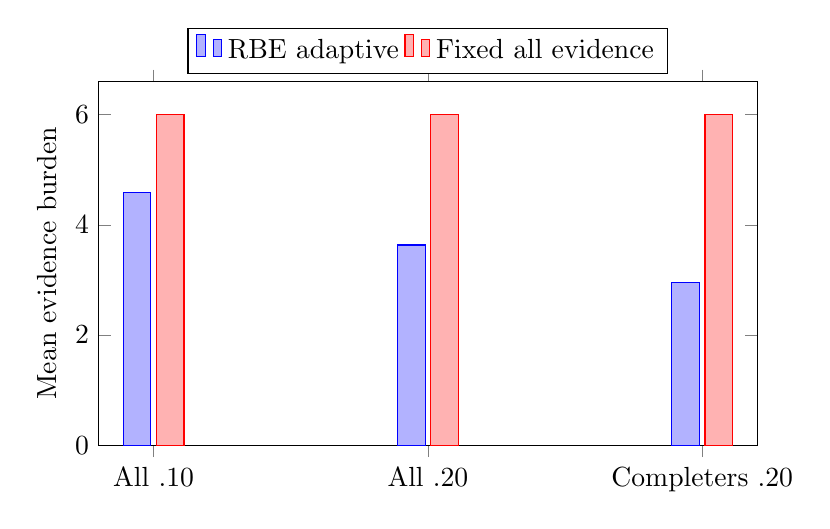
\begin{tikzpicture}
\begin{axis}[width=.82\textwidth,height=6.2cm,ybar,bar width=10pt,ylabel={Mean evidence burden},symbolic x coords={All .10,All .20,Completers .20},xtick=data,ymin=0,ymax=6.6,legend style={at={(0.5,1.02)},anchor=south,legend columns=2}]
\addplot coordinates {(All .10,4.5817) (All .20,3.6332) (Completers .20,2.9557)};
\addplot coordinates {(All .10,6) (All .20,6) (Completers .20,6)};
\legend{RBE adaptive,Fixed all evidence}
\end{axis}
\end{tikzpicture}
\caption{Evidence-burden comparison at matched selective coverage. Adaptive acquisition consistently uses fewer evidence channels, while risk superiority is not consistent. Source: RBE OULAD falsification artifact.}
\label{fig:ouladburden}
\end{figure}

\Cref{fig:ouladburden} visualizes the empirical contribution that remains after the stronger claim has been falsified. This distinction matters methodologically: negative controls narrow the theory to what the data actually support.

\section{Interpretation}
The results support three conclusions and reject two tempting overclaims.

First, CARG is a structural property of the pair $(g,\cA)$: a credential can demand a distinction that its assessment language cannot observe. The theorem does not depend on GenAI, but GenAI makes the failure more likely by increasing the set of latent capability configurations capable of producing similar artifacts. This is consistent with contemporary concerns about assessment validity and originality \parencite{luo2024policies,ali2026validity,bannister2025pandora}.

Second, the correct operational response to unresolved attribution is not necessarily ``ask more questions.'' RBE asks for the minimum perturbation that changes the predictions of worlds requiring different decisions. In practice, this may be a changed constraint, an intentionally flawed AI recommendation, a transfer problem, or a request to verify evidence. This stance connects naturally to evaluative judgement and appropriate reliance \parencite{bearman2024evaluative,passi2024reliance,zhai2024overreliance}.

Third, evidence burden is an educationally meaningful design variable. Assessment consumes learner and staff time. If two protocols reach the same declared decision standard, the one requiring less evidence is attractive, provided validity, fairness, and risk are not worsened. The OULAD study provides retrospective evidence that selective stopping can reduce evidence acquisition, but it cannot establish causal educational benefit.

Two claims are rejected. We do not claim that adaptive RBE is more accurate than enhanced fixed evidence; matched-coverage falsification does not support consistent dominance. We also do not claim that the present validation-learned evidence ordering is uniquely optimal; random-order controls occasionally match or outperform it. These negative results are retained because a framework for certification validity should itself tolerate falsification.

\section{Implications for Curriculum, Teaching, and Certification}
A practical RBE implementation begins with \emph{Resolvable Capability Outcomes} rather than task descriptions alone. A capability outcome should specify: (i) the capability claim, (ii) relevant environments, including permitted AI/tool conditions, (iii) admissible perturbations, and (iv) the certification distinction that matters. This extends constructive alignment \parencite{biggs1996alignment} by adding an explicit resolution criterion.

Learning and certification evidence should also be separated. During learning, hints, collaboration, retries, and AI support can be developmentally useful \parencite{black1998assessment,nicol2006feedback,hattie2007feedback}. Certification, however, requires evidence that supports the intended inference. A deliberately misleading AI suggestion can therefore be appropriate in a short resolution episode even if ordinary teaching encourages tool use, because the assessment purpose is to test whether the learner can discriminate reliable from unreliable support.

Finally, the framework supports a capability ledger rather than a single opaque grade: conceptual foundation, AI augmentation, verification, transfer, response to changed constraints, misleading-AI resistance, evidence revision, and minimum independent capability. Such a ledger should not be treated as a validated measurement scale without empirical work; it is a design architecture for making the evidentiary basis of certification more auditable.

\section{Limitations and Research Agenda}
The strongest limitation is empirical. OULAD predates GenAI and contains passive digital traces, not designed perturbations. Its final-result label is a proxy endpoint. Accordingly, the OULAD analysis validates software behavior and evidence-acquisition logic only; it cannot establish fairness, learning gains, causal effects, institutional superiority, or GenAI-specific validity.

The synthetic learner worlds are explanatory constructions. Their usefulness lies in exposing a logical failure mode and testing the code under known conditions, not in claiming psychological realism. Likewise, assessment leakage needs empirical operationalization: some perturbations provide information that may teach the learner while measuring them, an issue long recognized in dynamic assessment \parencite{allal2000zpd,poehner2011validity}.

A decisive prospective study should randomize or counterbalance conventional fixed assessment, enhanced authentic assessment, and adaptive RBE resolution episodes within the same course. Outcomes should include unseen transfer, error detection, misleading-AI resistance, calibration, inter-rater reliability, student/staff burden, subgroup invariance, and downstream performance. Risk--coverage curves should be reported rather than one favorable operating point. Any fairness claim should require explicit subgroup analysis and measurement-invariance work.

\section{Conclusion}
GenAI does not merely create an academic-integrity problem. It exposes an inference problem: high-quality observed work can be compatible with learner worlds that a credential should treat differently. RBE names the structural mismatch as a Certification--Assessment Resolution Gap and places a simple necessity condition beneath certification: assessment-indistinguishable worlds must not require different credential decisions.

The practical consequence is equally simple. When a gap remains, do not automatically expand the exam. Find the cheapest admissible perturbation that separates the certification-incompatible worlds still consistent with the evidence, and stop when the decision is resolved to the declared standard. The software experiments show why the constraint matters, why risk must accompany resolution, and why negative controls are essential. Real-data falsification does not support a claim that adaptive RBE is universally more accurate; it does support the narrower observation that adaptive selective assessment can reduce evidence burden. In the primary OULAD configuration, the mean saving was 2.37 evidence channels (39.45\%; 95\% percentile CI 2.31--2.42), while matched-coverage controls continued to block a predictive-superiority claim.

The central proposition is therefore not that outcomes cease to matter. It is that \emph{outcomes are not self-certifying}. In an AI-mediated university, the evidentiary question behind every credential becomes: \textbf{does the assessment resolve the capability distinction that the certificate claims to make?}

\section*{Data and Code Availability}
All software, tests, benchmark generators, workflow definitions, test registry entries, and saved result files used in this paper are available in the public repository: \url{https://github.com/Arithmetic-Power-Geometry/Resolution-Based-Education}. The repository is released under the Apache License 2.0 and records negative as well as positive results. OULAD is not redistributed; the benchmark retrieves the official public dataset and records its provenance \parencite{kuzilek2017oulad}.

\section*{Reproducibility Statement}
The deterministic and probabilistic experiments are fully specified by repository data and code. Monte Carlo experiments use the fixed seed 20260916. OULAD analyses use student-disjoint train/validation/test splits, validation-learned acquisition order, and held-out evaluation. The final burden uncertainty analysis uses 5,000 paired bootstrap resamples and was executed successfully in GitHub Actions workflow run 35074988489; artifact 10437304387 preserves the numerical output. The repository-wide test suite also passed after dependency repair in run 35074242019. The paper does not include an unverified result from any failed CI run.

\printbibliography
\end{document}
